% Part VI — Conclusion  |  ~8 slides  |  Madrid/seahorse  |  16:9
\documentclass[aspectratio=169,10pt]{beamer}
\usetheme{Madrid}\usecolortheme{seahorse}
\usepackage{tikz}
\usetikzlibrary{arrows.meta,shapes,positioning}
\usepackage{pgfplots}\pgfplotsset{compat=1.17}
\usepackage{booktabs,amsmath,amssymb,xcolor}
\definecolor{myblue}{RGB}{0,50,130}
\definecolor{myred}{RGB}{153,0,0}
\definecolor{mygreen}{RGB}{0,100,50}
\definecolor{myorange}{RGB}{180,80,0}
\newcommand{\NHOP}{\mathrm{NHOP}}
\newcommand{\TV}{\mathrm{TV}}
\setbeamertemplate{navigation symbols}{}
\title[Part VI: Conclusion]{Part VI — Synthesis and Conclusion}
\subtitle{Seven Contributions, Four Cross-Cutting Findings, and the Road Ahead}
\author{Parsa Hajiannejad}\date{2026}

\begin{document}
\begin{frame}\titlepage\end{frame}

% ----- Slide 1 ---------------------------------------------------------------
\begin{frame}{What Was Built and What Was Proved}
\begin{columns}[T]
\column{0.50\textwidth}
\textbf{Built:}
\begin{itemize}
  \item \textbf{NHOP}: distributional measure with exact TV identity and permutation test
  \item \textbf{Seed selection pipeline}: 4-stage, composite criterion; $+0.025$ F1 over random
  \item \textbf{GVM-CO / LRE-CO / LS-CO}: 3 circular algorithms; $+0.012$--$+0.015$ F1 over SMOTE
  \item \textbf{LeakageSafeCV}: prevents 2--5\% AUC inflation in benchmarks
  \item \textbf{Degradation-recovery protocol}: causally isolates IR from distributional shift
\end{itemize}

\column{0.48\textwidth}
\textbf{Proved empirically:}
\begin{center}
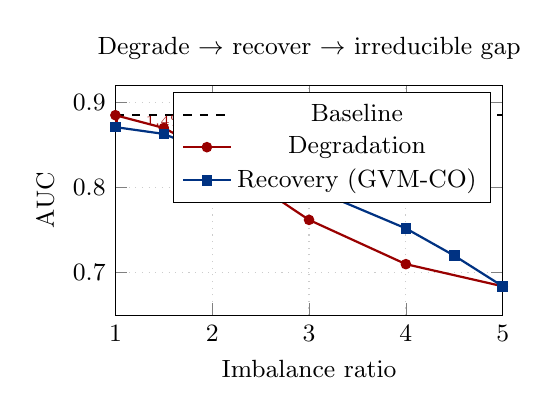
\begin{tikzpicture}
\begin{axis}[
  width=6.5cm,height=4.5cm,
  xlabel={\small Imbalance ratio},
  ylabel={\small AUC},
  xmin=1,xmax=5,ymin=0.65,ymax=0.92,
  xtick={1,2,3,4,5},
  xticklabel style={font=\small},
  yticklabel style={font=\small},
  xlabel style={font=\small},
  ylabel style={font=\small},
  title={\small Degrade $\to$ recover $\to$ irreducible gap},
  title style={font=\small},
  legend style={font=\small,at={(0.97,0.97)},anchor=north east},
  grid=major,grid style={dotted,gray!40}]
\addplot[dashed,black,thick,domain=1:5]{0.885};
\addplot[thick,myred,mark=*,mark size=1.5pt] coordinates {
  (1,0.885)(1.5,0.870)(2,0.840)(2.5,0.800)(3,0.762)(4,0.710)(5,0.684)};
\addplot[thick,myblue,mark=square*,mark size=1.5pt] coordinates {
  (5,0.684)(4.5,0.720)(4,0.752)(3,0.800)(2,0.840)(1.5,0.863)(1,0.871)};
\draw[myred,{Stealth[length=4pt]}-{Stealth[length=4pt]}] (axis cs:1,0.871)--(axis cs:1,0.885);
\node[font=\tiny,myred] at (axis cs:1.7,0.878) {1.4\% gap};
\legend{Baseline,Degradation,Recovery (GVM-CO)}
\end{axis}
\end{tikzpicture}
\end{center}
\end{columns}
\end{frame}

% ----- Slide 2 ---------------------------------------------------------------
\begin{frame}{Four Cross-Cutting Findings}
\begin{center}
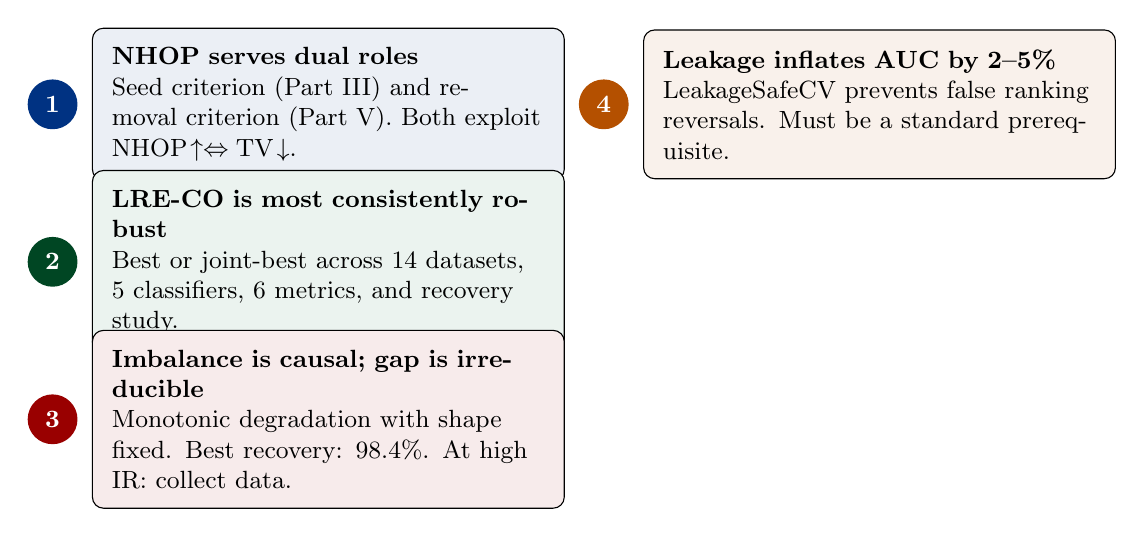
\begin{tikzpicture}[
  fbox/.style={rectangle,rounded corners=4pt,draw,text width=5.5cm,
               align=left,font=\small,inner sep=7pt},
  num/.style={circle,fill,text=white,font=\bfseries\small,minimum size=18pt,inner sep=0pt}]
\node[num,fill=myblue]  (n1) at (0,0)    {1};
\node[fbox,right=5pt of n1,fill=myblue!8] (f1) {%
  \textbf{NHOP serves dual roles}\\
  Seed criterion (Part III) and removal criterion (Part V). Both exploit $\NHOP\!\uparrow\Leftrightarrow\TV\!\downarrow$.};

\node[num,fill=mygreen!70!black] (n2) at (0,-2.0) {2};
\node[fbox,right=5pt of n2,fill=mygreen!8] (f2) {%
  \textbf{LRE-CO is most consistently robust}\\
  Best or joint-best across 14 datasets, 5 classifiers, 6 metrics, and recovery study.};

\node[num,fill=myred] (n3) at (0,-4.0) {3};
\node[fbox,right=5pt of n3,fill=myred!8] (f3) {%
  \textbf{Imbalance is causal; gap is irreducible}\\
  Monotonic degradation with shape fixed. Best recovery: 98.4\%. At high IR: collect data.};

\node[num,fill=myorange] (n4) at (7,0) {4};
\node[fbox,right=5pt of n4,fill=myorange!8] (f4) {%
  \textbf{Leakage inflates AUC by 2--5\%}\\
  LeakageSafeCV prevents false ranking reversals. Must be a standard prerequisite.};
\end{tikzpicture}
\end{center}
\end{frame}

% ----- Slide 3 ---------------------------------------------------------------
\begin{frame}{Limitations and Future Work}
\begin{columns}[T]
\column{0.50\textwidth}
\textbf{Known limitations:}
\begin{itemize}
  \item NHOP is \emph{marginal}: misses joint dependencies across features
  \item Benchmark: $N=14$ datasets — power $\approx 30\%$ for rank-2 effects ($N\geq45$ needed)
  \item Causal study: $\IR\leq4$ only; binary classification only
  \item Native-mode VMF accuracy degrades at $d>100$
\end{itemize}

\column{0.48\textwidth}
\textbf{Future directions:}
\begin{itemize}
  \item Multivariate NHOP via copula decompositions (joint dependencies)
  \item Extend benchmark to $N\geq45$ for 80\% power
  \item Multi-class imbalance and extreme IR ($\leq50$)
  \item Oversampler targeting the irreducible gap via uncertainty quantification
  \item NHOP-guided active learning: prioritise minority collection by marginal NHOP gain
\end{itemize}

\vspace{6pt}
\textbf{Unified vision:} a closed-loop production system where NHOP monitors minority coverage, triggers GVM-CO synthesis when coverage drops, and active learning prioritises data collection — calibrated by the causal recovery curves.
\end{columns}
\end{frame}

% ----- Slide 4 (closing) -----------------------------------------------------
\begin{frame}[plain]
\begin{center}
\vspace{1.0cm}
{\Huge\color{myblue} Thank You}
\vspace{0.8cm}

{\large\color{myblue!70!black} NHOP $\cdot$ Seed Selection $\cdot$ Circular Oversampling $\cdot$ Causal Evidence}

\vspace{0.7cm}
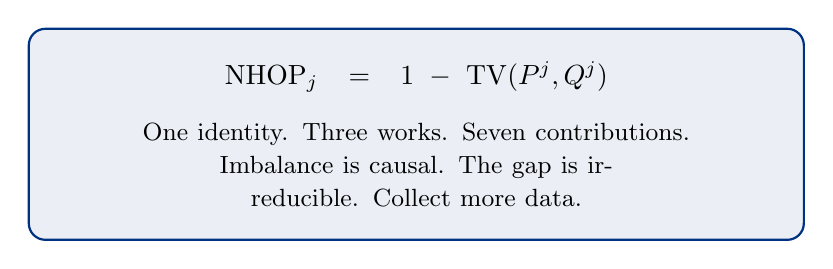
\begin{tikzpicture}
\node[draw=myblue,thick,rounded corners=6pt,fill=myblue!8,
      text width=9cm,align=center,font=\normalsize,inner sep=12pt]{%
  $\NHOP_j = 1 - \TV(P^j, Q^j)$\\[8pt]
  {\small One identity. Three works. Seven contributions.}\\
  {\small Imbalance is causal. The gap is irreducible. Collect more data.}
};
\end{tikzpicture}
\end{center}
\end{frame}

\end{document}
